\section{Média Aritmética Simples e Ponderada}


\quest{Oficial de Justiça 2023 - VUNESP}{O gráfico apresenta o número de acertos na prova de Língua Portuguesa e de Matemática, aplicada a dois candidatos, A e B, em um concurso interno para promoção de cargo:\\
	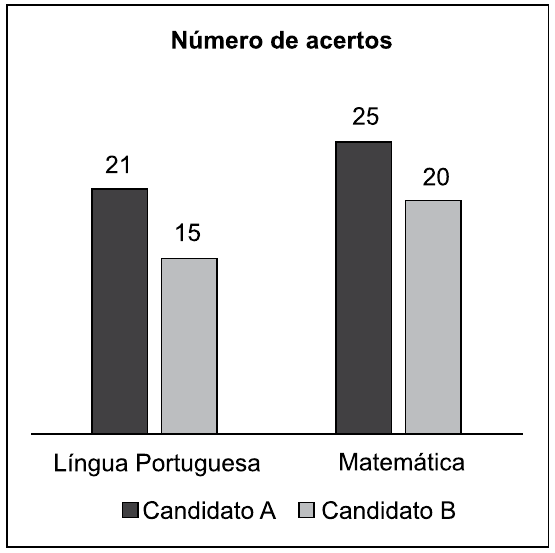
\includegraphics[scale=.5]{fig001.png}\\
Sabendo-se que a prova de Língua Portuguesa tinha 	peso 2 e a de Matemática tinha peso 3 para o cargo em 	concurso, que cada uma das provas tinha 50 questões, 	e que a nota de cada prova é igual ao número de acertos correspondente, é correto afirmar que o número de questões de Matemática que o candidato B deveria ter acertado a mais, para que a média aritmética ponderada das notas das suas provas fosse igual à média aritmética ponderada das notas das provas do candidato A, é igual a}
{\item 9.
\item 20.
\item 10.
\item 29.
\item 27.}
{https://youtu.be/BvsQZctqarQ}
